\documentclass[times, utf8, diplomski, numeric]{fer}
\usepackage{booktabs}
\usepackage{nameref}

\newcommand{\norm}[1]{\left\lVert#1\right\rVert}
\newcommand{\abs}[1]{\left\lvert#1\right\rvert}

\begin{document}

% TODO: Navedite broj rada.
\thesisnumber{1147}

% TODO: Navedite naslov rada.
\title{Semantička segmentacija prirodnih scena dubokim neuronskim mrežama}

% TODO: Navedite vaše ime i prezime.
\author{Ivan Borko}

\maketitle

% Ispis stranice s napomenom o umetanju izvornika rada. Uklonite naredbu \izvornik ako želite izbaciti tu stranicu.
\izvornik

% Dodavanje zahvale ili prazne stranice. Ako ne želite dodati zahvalu, naredbu ostavite radi prazne stranice.
\zahvala{}

\tableofcontents

\chapter{Uvod}

Razumijevanje scene osnovni je problem mnogih segmenata računalnog vida. Jedan od načina na koji se može ostvariti razumijevanje scene je semantička segmentacija, odnosno proces pridjeljivanja semantičkih oznaka dijelovima scene. Primjeri oznaka su: nebo, more, livada, stablo, automobil, osoba, zgrada. Scena je obično predstavljena digitalnom fotografijom pa onda govorimo o pridjeljivanju oznaka svakom pikselu.

Razumijevanje scene bitan je dio mnogih autonomnih robotiziranih sustava koji čine interakcije s okolinom.
Primjer su autonomni automobili koji su u zadnje vrijeme postigli veliki razvojni napredak pa često svjedočimo reportažama o vožnjama ili pak testovima novih prototipova. Takvi automobili koriste sustave za razumijevanje scene kako bi pratili cestu kojom voze, pratili druge sudionike u prometu i mogli izbjeći potencijalne nesreće.

Ovaj rad opisuje sustav za semantičku segmentaciju koji koristi već segmentirane scene za "učenje" svojih parametara. Arhitektura sustava se temelji na dubokim neuronskim mrežama, konkretno konvolucijskim neuronskim mrežama. Sustavi temeljeni na konvolucijskim mrežama postižu najbolje rezultate \engl{state-of-the-art} u mnogim zadacima računalnog vida poput klasifikacije (\cite{krizhevsky_imagenet}, \cite{googlenet}, \cite{vgg_net}, \cite{overfeat}), detekcije objekata (\cite{girshick2014rcnn}), fine kategorizacije \engl{fine grained categorization}(\cite{zhang14finegrained}) i semantičke segmentacije (\cite{farabet_pami}, \cite{long_shelhamer}, \cite{ChenPKMY14}).

Do prije četiri godine godine konvolucijske mreže nisu bile glavni alat za semantičku segmentaciju. Tada su se uglavnom koristile razne metode temeljene na grafovima i grupiranju piksela u skupine. U takvim postupcima često se za svaku regiju od 8x8 piksela računaju HOG \engl{histogram of gradients} ili SIFT \engl{scale invariant feature transform} opisnici \cite{Lowe:1999}. Ti opisnici predstavljaju značajku te regije i ulaze u klasifikator koji ih zatim grupira i klasificira.
Korištenjem klasifikatora poput stabala odluke ili šumama tekstona optimira se 
Ako se koriste klasifikatori temeljeni na stablima odluka ili šumama tekstona onda klasifikator ima svoju energetsku funkciju koju optimira tako da je je slika optimalno pokrivena semantičkim oznakama.

Opisi poglavlja...

\chapter{Neuronske mreže}

Umjetne neuronske mreže \engl{artificial neural networks} ili skraćeno neuronske mreže su paradigma koja opisuje procesiranje informacija inspirirano načinom na koji ljudski mozak (promatran samo kao skup neurona) procesira informacije, odnosno električne impulse. Glavna odlika neuronske mreže je procesiranje informacija jednostavnim elementima (neuronima) na visokoj razini paralelizma. Ti jednostavni elementi su međusobno povezani velikim brojem veza (u biološkom sustavu te veze su sinapse). Učenje neuronskog biološkog sustava podrazumijeva podešavanje sinapsi, a slično tome se podešavaju parametri u umjetnoj neuronskoj mreži.

Osnovni element umjetne neuronske mreže je umjetni neuron. Prvi umjetni neuron, nazvan perceptron, razvio je Frank Rosenblatt 1950-ih inspiriran ranijim radom \cite{mcculloch43a}  Warrena  McCullocha i Waltera Pittsa iz 1943. o njihovom viđenju umjetnog neurona. Taj početni entuzijazam nije predugo trajao jer Minsky i Papert 1969. godine objavljuju knjigu \cite{minsky69perceptrons} u kojoj navode mane neuronskih mreža i daju pesimističan pogled na neuronske mreže. Tada većina znanstenika prestaje s istraživanjima na tome polju i razvoj ostaje na par znanstvenika koji su trebali dokazati mogućnosti neuronskih mreža.

\begin{figure}[htb]
\centering
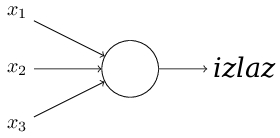
\includegraphics{imgs/percep.png}
\caption{Primjer perceptrona s 3 ulaza}
\label{fig:percep}
\end{figure}

Slika \ref{fig:percep} prikazuje primjer perceptrona koji ima 3 ulaza, $x_1, x_2, x_3$. Općenito, broj ulaza je proizvoljan. Rosenblatt je predstavio pravilo kako se računa izlaz iz neurona: postoje težine $w_1, w_2, ...$, realni brojevi koji predstavljaju značaj pripadajućih ulaza. Izlaz neurona se određuje prema tome je li suma $\sum_{j} w_j * x_j$ veća ili manje od neke fiksne vrijednost. Matematički se to može zapisati kao:
\begin{equation}
izlaz =
\left\{
	\begin{array}{ll}
		0  & \mbox{ako } \sum_j w_j * x_j \leq prag \\
		1  & \mbox{ako } \sum_j w_j * x_j >  prag
	\end{array}
\right.
\end{equation}

Učenje takvog modela se zapravo svodi na podešavanje težina $w_j$ i praga, čime se postižu različite vrijednosti izlaza.

Današnji umjetni neuron koji se koristi u neuronskim mrežama se malo razlikuje od originalne ideje perceptrona po tome što ne koristi step funkciju na izlazu, već neku funckciju iz porodice sigmoidalnih funkcija (neki autori takav neuron nazivaju logistički neuron ili logistički perceptron).

No, nije samo rad Minskog i Paperta kočio razvoj neuronskih mreža: računalna snaga je tada bila veliko ograničenje. Zato su se proučavali tek jednostavni modeli, koji nisu imali dovoljnu moć. Prava moć dolazi tek kada se više perceptrona spoji zajedno kroz više slojeva (vidi Višeslojni perceptron). Tokom 80-ih godina dolazi do razvoja računalnog paralelizma i povećanja računalne snage čime rastu mogućnosti za treniranje i evaluacije kompleksnijih neuronskih mreža.

Značajan napredak postigao je i Werbos 1975. godine kada je u svojem radu \cite{Werbos:74} primjenio algoritam unazadne propagacije \engl{backpropagation} za učenje neuronskih mreža (vidi poglavlje Backgropagation).
Često se taj trenutak naziva i renesansom neuronskim mreža jer opisani postupak omogućava lako treniranje neuronskih mreža neovisno o njihovoj složenosti i arhitekturi.

Za to vrijeme snažno su se razvijali drugi algoritmi strojnog učenja. Stroj s potpornim vektorima \engl{support vector machine}, ili kraće SVM, tako postaje moćniji i zastupljeniji klasifikator od neuronskih mreža. Tek zadnjih 10-ak godina duboke neuronske mreža polako preuzimaju primat SVM-a zbog dolaska GPGPU \engl{general purpose graphics processsing unit} jedinica koje su sposobne izvršavati velike količine paraleliziranih matričnih operacija potrebnih za treniranje dubokih mreža.

\section{Klasifikacija i regresija}
Dva temeljna problema prediktivnih sustava su klasifikacija i regresija.
Klasifikacija je razvrstavanje ulaznih podatka u jedan od $K$ razreda. Ako je $K = 2$ onda govorimo o binarnoj klasifikaciji. Kod neuronskih mreža se to može ostvariti postavljanjem step funkcije na na kraj zadnjeg neurona čime izlaz postaje $0 / 1$.
Za razliku od klasifikacije, regresija daje realni broj kao izlaz. Cilj je da realni izlaz bude čim sličniji traženom izrazu.

\section{Nadzirano i nenadzirano učenje}
Dva su glavna pristupa učenju prediktivnih modela koja vrijede i za neuronske mreže: nadzirano i nenadzirano učenje. Tokom nadziranog učenja mreži prezentiramo par podataka $(x, y), x \in X, y \in Y$, gdje je X skup svih ulaza u mrežu, a Y skup pripadnih izlaznih (traženih) vrijednosti.
Cilj je pronaći funkciju $f: X \to Y$, koja aproksimira preslikavanje implicirano u podacima za učenje.

Parametri modela se optimiraju tako da se smanjuje zadana funkcija troška \engl{cost function}. Funkcija troška može biti srednja kvadratna pogreška između traženih i dobivenih vrijednosti na izlazu (većinom korištena za regresijske probleme),
\begin{equation}
	\mathcal{L} = (y_t - y_p)^2
\end{equation}
ili pak pogreška unakrsne entropije (većinom korištena za klasifikaciju)
\begin{equation}
	\mathcal{L} = -\log P(y_p | y_t) = -(y_t \log(y_p) + (1 - y_t) \log(1 - y_p))
\end{equation}

gdje je $y_t$ je tražena vrijednost na izlazu, a $y_p$ je dobivena (predviđena) vrijednost.

Tokom nenadziranog učenja nema izlaznog skupa podataka, samo ulazni skup $X$. Dana je i funkcija troška koja se optimira. Cilj može biti grupiranje podataka u $K$ grupa pa je tada funkcija troška određena mjera disperzije uzoraka unutar grupe. Ili se pak traži kompresija ulaznog višedimenzionalnog vektora u manje dimenzionalan pa je funkcija troška zapravo pogreška rekonstrukcije.

\section{Logistička regresija}
\label{chap:logisticka_regresija}

Originalni perceptron se razvijao kroz povijest i njegova verzija koja se trenutno koristi u neuronskim mrežama izgleda malo drugačije. Ulazi više ne moraju biti binarne vrijednosti, već to mogu biti realne vrijednosti, a funkcija na izlazu je sigmoid (logistička funkcija), definirana formulom:
\begin{equation}
f(x) = \frac{1}{1+e^{-x}}
\end{equation}

Takav se model naziva logistička regresija. Logistička regresija je jedan od osnovnih klasifikacijskih modela, iako joj ime govori da je to regresijski model, što ona nije. Ona je probabilistički (njezin izlaz predstavlja vjerojatnost da je primjer u određenom razredu) i linearni klasifikator (decizijska granica je linearna)\cite{strojno_snajder}. Kod jednostavne (dvoklasne) klasifikacije parametri logističke regresije su vektor težina $\boldsymbol{w}$ i pomak $\boldsymbol{b}$. Ako govorimo o višeklasnoj klasifikaciji, parametri logističke regresije su matrica težina $\boldsymbol{W}$ i vektor pomaka $\boldsymbol{b}$. Klasifikacija se vrši tako da se određuje projekcija točaka u n-dimenzionalnom prostoru na hiperravnine koje predstavljaju granice između razreda uzoraka.

Matematički se to može zapisati kao:
\begin{equation}
P(Y = 1 | \boldsymbol{x}, \boldsymbol{w}, b) = f(\boldsymbol{w}*\boldsymbol{x} + b) = \frac{1}{1+e^{-(\boldsymbol{w}*\boldsymbol{x} + b)}}
\label{eq:sigmoid}
\end{equation}
gdje je $f$ sigmoidalna funkcija, $\boldsymbol{x}$ ulazni vektor, a $Y$ je skup izlaznih vrijednosti (1 znači da pripada nekom razredu).

Odnosno kao
\begin{equation}
P(Y = i | \boldsymbol{x}, \boldsymbol{w}, b) = \mathrm{softmax}(\boldsymbol{w}*\boldsymbol{x} + b) = \frac{e^{\boldsymbol{x}^{\top} * \boldsymbol{w_i}}}{ \sum_{k=1}^K  e^{\boldsymbol{x}^{\top} * \boldsymbol{w_k}}}
\label{eq:softmax}
\end{equation}
za višeklasnu klasifikaciju ($i$ je oznaka klase kojoj pripada primjer $\boldsymbol{x}$).

Izlaz modela je tada jednak:
\begin{equation}
h = \arg\max_i P(Y = i|\boldsymbol{x}, \boldsymbol{w}, b)
\label{eq:model_out_arg}
\end{equation}

Želimo da klasifikator modelira vjerojatnosnu distribuciju primjera iz skupa $\mathcal{D}$. Kako bi se to postiglo, potrebno je podesiti težine i pomak. Uvodimo oznaku $\theta$, koja označava skup svih parametara modela (težine i pomak). Koristeći tu notaciju, možemo reći da modeliramo vjerojatnost primjera uvjetovanu skupom parametara:

\begin{center}
$P(x|\theta)$
\end{center}

Pošto nam je već poznata distribucija primjera $\mathcal{D}$, a zanimaju nas parametri $\theta$, uvodimo termin izglednost \engl{likelihood}, koju ćemo označiti simbolom $\mathcal{L}$. Izglednost parametara uvjetovana primjerom jednaka je vjerojatnosti tog primjera uvjetovanoj parametrima:

\begin{center}
$\mathcal{L}(\theta|x) = P(x|\theta)$
\end{center}

Razmotrimo značenje predočenog izraza. Poanta nije u procjeni točne vjerojatnosti, već u ideji da ako mjenjamo parametre $\theta$ tako da oni povećavaju vjerojatnost pojavljivanja primjera $x$ (desna strana izraza), tada time istovremeno povećavamo izglednost da su parametri $\theta$ baš oni koje tražimo (lijeva strana).

Ista ideja primjenjiva je na cijeli skup primjera za učenje $\mathcal{D}$. Pretpostavimo da su primjeri za učenje uzorkovani iz samo jedne distribucije. Pretpostavimo nadalje da su uzorci međusobno nezavisni . Tada govorimo o podatcima koji su nezavisni i identično distribuirani, za što se u literaturi često koristi akronim \emph{iid} \engl{independent, identically distributed}. Ako je zadovoljen \emph{iid} uvjet, možemo definirati vjerojatnost cijelog skupa za učenje $\mathcal{D}$:
\begin{center}
$P(\mathcal{D}) \overset{iid}{=} P(x)$
\end{center}

Iz dobivene vjerojatnosti $P(\mathcal{D})$, možemo definirati izglednost parametara s obzirom na cijeli skup za učenje $\mathcal{D}$:

\begin{equation}
\mathcal{L}(\theta|D) = P(D|\theta) \overset{iid}{=} \prod_{x \in D} P(x|\theta)
\end{equation}

Pošto u pravilu znamo za vjerojatnost $P(x|\theta)$, promjenom parametara $\theta$  možemo mijenjati vjerojatnost $P(\mathcal{D}|\theta)$. Tražimo skup parametara koji dotičnu vjerojatnost maksimizira. Za logističku regresiju to bi značilo da smo pronašli težine ($\boldsymbol{w}$) i pomak ($b$) koji dobro modeliraju skup primjera $\mathcal{D}$. Za pronalazak maksimuma vjerojatnosti $P(\mathcal{D}|\theta)$ koristimo gradijentni uspon.

Još preostaje za objasniti često korišteni trik kod maksimizacije vjerojatnosti. Razmotrimo logaritamsku funkciju $ln(x)$. Ona je rastuća na cijeloj domeni: povećanjem argumenta x, povećava se vrijednost funkcije $ln(x)$. Pošto se računica izglednosti odvija na intervalu $P(x) \in [0, 1]$, unutar domene logaritamske funkcije (izuzevši rubnu vrijednost 0, što nije problem), znamo da povećanjem $P(x)$ raste i $ln(P(x))$. Stoga umjesto maksimizacije izglednosti možemo koristiti maksimizaciju log-izglednosti:
\begin{equation}
ln \mathcal{L}(\theta|D) = ln P(D|\theta) \overset{iid}{=} ln \prod_{x \in D} P (x|\theta) = \sum_{x \in D} ln P (x|\theta)
\end{equation}

Maksimizacijom log-izglednosti pronalazimo isti skup parametara $\theta$ kao i maksimizacijom obične izglednosti, ali matematički izračun često bude jednostavniji.

Vratimo se sada na logističku regresiju. Za ulazni skup podataka, možemo definirati log izglednost $\mathcal{L}$ i gubitak $\ell$:
\begin{equation}
\mathcal{L} (\theta = \{\boldsymbol{w}, b\} | D) = \sum_{i=0}^{|D|} ln(P(Y = y^{(i)} | x^{(i)}, \boldsymbol{w}, b))
\label{eq:logistic_likelihood_func}
\end{equation}
\begin{equation}
\ell = (\theta = \{\boldsymbol{w}, b\} | \mathcal{D}) = -\mathcal{L}(\theta = \{\boldsymbol{w}, b\} | \mathcal{D})
\label{eq:logistic_loss_func}
\end{equation}

% TODO prebaci ovo u poglavlje Gradijentni spust
Da bi se algoritam gradijentnog spusta mogao koristiti, potrebno je derivirati funkciju gubitka. Kao prvo, nužno je da je ona derivabilna što je slučaj kod logističke regresije jer se kao prijenosna funkcija $f(x) = \frac{1}{1+e^{-x}}$ koristi logistička sigmoid funkcija. Alati poput Theano-a imaju mogućnost da se funkcija gubitka zada simbolički pa sami alati izvode deriviranje.

\url{http://deeplearning.net/software/theano/tutorial/gradients.html}

Obično se koristi metoda gradijentnog spusta nazvana stohastički gradijentni spust. Neka je $\ell_i(w)$ vrijednost funkcije gubitka na i-tom primjeru za neke parametre $w$.

Kada bi za minimizaciju koristili standardni (ili ''grupni'') gradijentni spust, jedna bi iteracija izgledala ovako:
\begin{equation}
    w := w - \alpha \nabla \ell(w) = w - \alpha \sum_{i=1}^n \nabla \ell_i(w),
\end{equation}
gdje je $\alpha$ korak učenja (često zvan i stopa učenja).

U mnogo slučajeva, funkcija nad kojom se vrši zbrajanje ima jednostavan oblik koji omogućava brzo izračunavanje zbrajanje i cijelog izraza.

No, postoje funkcije kod kojih izračuvanje sume u gradijentu zahtijeva dugotrajne izračune. Kad je skup za treniranje velik, to postaje problem. Da bi se ubrzalo izvođenje izračuna, u svakoj iteraciji se izvodi gradijenti spust, odnosno izračun funkcije gradijenta. Takvim se postupkom aproksimira pravi gradijent funkcije gubitka gradijentom jednog primjera (jedne iteracije):
\begin{equation}
    w := w - \alpha \nabla \ell_i(w).
\end{equation}
Prolazom algoritma kroz skup za treniranje izvodi se gornje podešavanje težina za svaki primjer. Potrebno je nekoliko prolaza kroz skup za treniranje dok algoritam ne konvergira. Tipične implementacije još i promješaju skup za učenje prije svakog prolaza.


\section{Višeslojni perceptron}
\label{chap:viseslojni_perceptron}

Do sada spomenuti modeli i arhitekture modeliraju samo jedan biološki neuron, dok je neuronska mreža skup neurona. Spajanjem više modela neurona u više slojeva (u dubinu) i više neurona u širinu, nastaje neuroska mreža. Najjednostavniji model neuronske mreže naziva se višeslojni perceptron.

Višeslojni perceptron se sastoji od 3 sloja: ulaznog sloja, skrivenog sloja \engl{hidden layer} i izlaznog sloja. Ulazni sloj se sastoji od brojeva koji opisuju neki primjer (vektor značajki nekog primjera), skriveni sloj se sastoji od logističkih neurona i zadnji sloj koji se također sastoji od logističkih neurona (broj izlaznih neurona ovisi o broju razreda u koji se klasificira primjer).

Višeslojni perceptron (slika \ref{fig:mlp}) se može promatrati i kao vrsta logističke regresije kod koje su ulazi transformirani pomoću nelinearne transformacije. Svrha tih transformacija je prebaciti ulazne podatke u prostor više dimenzije gdje oni postaju linearno separabilni (budući da je logistička regresija linearni klasifikator). Transformacije izvodi skriveni sloj i on je dovoljan da MLP postane univerzalni aproksimator.

\begin{figure}[htb]
\centering
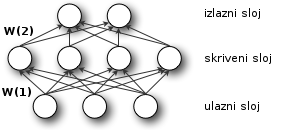
\includegraphics{imgs/mlp.png}
\caption{Višeslojni perceptron}
\label{fig:mlp}
\end{figure}

Izlaz višeslojnog perceptrona je tada:
\begin{equation}
f(\boldsymbol{x}) = G\{\boldsymbol{W}(2) * (s[\boldsymbol{W}(1) * \boldsymbol{x} + \boldsymbol{b}(1))] + \boldsymbol{b}(2)\}
\label{eq:conv}
\end{equation}
$G$ i $s$ su aktivacijske funkcije. Za aktivacijsku funkciju se obično odabire logistička sigmoid funkcija ili $\tanh$. $\tanh$ se odabire jer se višeslojna mreža s njime kao prijenosnom funkcijom brže trenira.
Jednadžba se može protumačiti na način da se izlaz skrivenog sloja $h(\boldsymbol{x}) = s( \boldsymbol{W}(1) * \boldsymbol{x} + \boldsymbol{b} )$ prosljeđuje na ulaz logističke regresije, čime dobijemo višeslojni perceptron.

\section{Duboke neuronske mreže}

Duboke neuronske mreže (ili kraće, DNN) su naziv za neuronske mreže koje sadrže dva ili više skrivena sloja. Takve duboke mreže omogućuju modeliranje komplesnih nelinearnih zavisnosti, poput viešeslojnog perceptrona. Zbog velike količine parametara i same dubine, dugo vremena je treniranje takve mreže bilo problematično, no u zadnjih nekoliko godina, razvile su se metode za njihovo treniranje, ali i same arhitekture koje imaju puno manji broj parametera, a jednaku dubinu i širinu.

Recimo da se želi konstruirati sustav za prepoznavanje lica na slici. Mogli bi koristiti jedan model višeslojnog perceptrona koji bi odgovorio na pitanje postoji li oko slici, drugi model koji bi pak odgovorio na pitanje postoje li usta na slici, treći model koji bi odgovorio postoji li kosa na slici. Izlaze tih modela bi mogli spojiti na logističku regresiju koja koristi sve izlaze postojećih modela i vraća odgovor postoji li lice na slici. Duboke neuronske mreže mogu zamijeniti takav složeni sustav, jer omogućuju spajanje više slojeva koji se specijaliziraju za različite dubine apstrakcije, a treniranje i korištenje dubokih mreža je jednostavnije od navednog skupa modela.

DNN su obično dizajnirane kao mreže s unaprijednom propagacijom, no posljednja istraživanja pokazuju da je moguće koristiti i neuronske mreže s povratom \engl{recurrent networks} u dubokim arhitekturama (primjer je modeliranje jezika). Jedna specifična verzija dubokih neuronskih mreža su konvolucijske neuronske mreže koje su vrlo često korištene u računalnom vidu (detaljno opisane u poglavlju \ref{chap:konvolucijske_mreze}).

Pokazalo se da je proces treniranja dubokih neuronskih mreža iznimno težak. Algoritmi bazirani na gradijentnim metodama skloni su pronalasku lokalnih optimuma. Drugi je problem nestajući gradijent \engl{vanishing gradient problem} koji se dešava tokom unazadne propagacije gradijenata jer se iznos gradijenata smanjuje za red veličine po sloju što znači da se gradijent teško prenosi do prednjih slojeva.

Nadalje, iole kompleksnije mreže su vrlo teške za interpretaciju, čak i ako rade dobro, količina parametara je toliko ogromna da je mreža zapravo ''crna kutija'' i nemoguće je analizom ustvrditi zašto dobro rade.

U zadnjih desetak godina slojevitim umjetnim neuronskim mrežama pristupa se
na novi način. Radi se s nekoliko tehnika koje imaju par zajedničkih aspekata.
Kod nekih tehnika (autoenkoderi, ograničeni Boltzmanovi strojevi) slojevi se treniraju jedan po jedan, dok kod drugih (konvolucijske mreže) postoji posebna vrsta slojeva koji imaju smanjen broj parametara i rijetko su povezani čime je smanjen broj operacija po sloju.

Kao zajedničko ime za više tehnika koje na ovaj način pristupaju treniranju umjetne neuronske mreže koristi se termin "duboka neuronska mreža". Duboke neuronske mreže na tipičnim klasifikacijskim problemima postižu rezultate koji su među ponajboljima ikad postignutim.

\subsection{Autoenkoderi}

Autoenkoderi su posebna vrsta umjetnih neuronskih mreža koje se koriste za učenje prikaza informacija u manje memorije (sažimanje), na što se može gledati i kao na metodu smanjivanja značajki ulaznog prostora.
Osnovna ideja autoenkodera je poprilično jednostavna: imamo neuronsku mrežu kojoj ulazni i izlazni sloj imaju jednak broj neurona, u sredinu dodamo još jedan sloj s manjim brojem neurona. Taj srednji sloj, koji je zapravo ''usko grlo'' će naučiti efikasno prikazati ulaze podatke (kodirati ih).

Najjednostavniji model autoenkoderske mreže ima, kao što je već spomenuto, tri sloja (poput MLP-a, poglavlje \ref{chap:viseslojni_perceptron}): ulazni, skriveni i izlazni. Skriveni sloj ima manje neurona od ulaznog, jer se prebacivanjem iz ulaznog u skriveni vrši sažimanje. Postupkom treniranja se nastoji postići da informacija koja dođe na ulazni sloja ($\boldsymbol{x}$) čim sličnija izađe iz izlaznog sloja ($\hat{\boldsymbol{x}}$). Iz toga slijedi da izlazni i ulazni sloj moraju imati jednak broj neurona. Pogreška rekonstrukcije ($\Delta \boldsymbol{x} = \boldsymbol{x} - \hat{\boldsymbol{x}}$) se koristi za podešavanje težina u mreži.
\begin{figure}[htb]
\centering
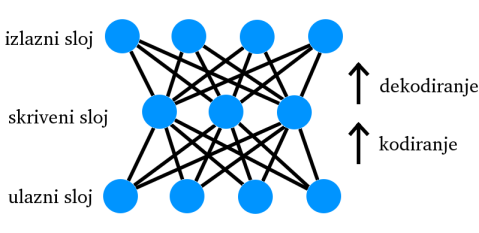
\includegraphics{imgs/autoencoder.png}
\caption{Jednostavni autoenkoder s jednim skrivenim slojem}
\label{fig:autoencoder}
\end{figure}

Hinton je u radu \cite{hinton_autoencoder} prvi upotrijebio autoenkodere kao metodu treniranje dubokih neuronskih mreža. Takvim se treniranjem svaki sloj redom uzima kao skriveni sloj autoenkodera i trenira. Na kraju se cijela mreža nastala od tako istreniranih slojeva spaja i rezultirajuća se mreža fino ugađa primjenom postojećih gradijentnih tehnika.
Treniranjem slojeva pojedinačno poboljšava se pretraga parametarskog prostora mreže: bolje se izbjegavaju lokalni optimumi. Moguće je efikasno trenirati više slojeva koji sadrže veći broj neurona, što omogućava stvaranje puno kompleksnijih mreža koje se dobro nose s težim zadatcima. Niži slojevi mogu se trenirati sa neoznačenim podatcima (polu-nadzirano učenje).

\section{Konvolucijske neuronske mreže}
\label{chap:konvolucijske_mreze}

Duboke neuronske mreže koje sadrže konvolucijske slojeve (pojašnjeni u sljedećem poglavlju) nazivaju se konvolucijskim neuronskim mrežama. Konvolucijske mreže se danas primjenjuju u većini problema računalog vida gdje vrlo često postižu vrhunske rezultate.

\subsection{Konvolucijski sloj}

Znanstveni radovi temeljeni na vidnom korteksu \engl{visual cortex} mačaka pokazali su da postoji složeni raspored vidnih stanica u oku. Neke od tih stanica osjetljive su na samo malu podregiju vidnog polja nazvanu osjetilno polje \engl{receptive field}. Takve su stanice raspoređene da pokrivaju cijelo vidno polje. Dodatno, identificirana su dva tipa stanica: jednostavne stanice i kompleksne stanice. Jednostavne maksimalno reagiraju na podražajne oblike s izraženim bridovima dok složene imaju veća osjetilna područja i invarijantne su na točnu poziciju podražaja.

Budući da je vizualni korteks trenutno najmoćniji sustav vida, čini se logičnim pokušati emulirati njegovo ponašanje. Mnogi takvi sustavi se mogu pronaći u literaturi, poput sustava NeoCognitron \cite{neocognitron} i mnogih drugih \cite{cortex_mehachanism} \cite{gradient_document}.

Konvolucija je matematički pojam, definiran kao učestalo primjenjivanje funkcije na podacima. U ovom konktekstu to znači primjenjivati ''filter'' na sliku po svim mogućima pomacima, oponašajući osjetilne stanice u ljudskom oku. Filter predstavlja skup težina povezanih sa prethodnim slojem, gdje je prethodni sloj komadić 2-D ulazne slike, a izlaz je jedan neuron. Takav se filter primjenjuje pomičući kroz cijelu sliku, pri čemu se ''osjetilna polja''' preklapaju, kao što je prikazano na slici \ref{fig:sparse-nn} te nastaje nova 2-D matrica koja se naziva mapa značajki. Jedan konvolucijski sloj sadrži više takvih filtera što ima za posljedicu da nastaje i više mapa značajki.

U zadacima računalnog vida posebno se osjeti rast parametara s dubinom i širinom mreže jer se na ulazu nalaze slike (u digitalnom obliku), dimenzija često preko 100x100 piksela (relativno mala slika), što daje 10 000 značajki na ulazu i čini ulazni prostor visoko dimenzionalnim. Uzmimo za primjer mrežu sa 10 000 ulaznih neurona i 1000 skrivenih neurona. Takav prvi sloj ima već 10 milijuna težina, a slaganjem mreže u dubinu se taj broj još povećava, mreža se teško i sporo trenira te je sklona prenaučenosti.

%(slika http://deeplearning.net/tutorial/_images/sparse_1D_nn.png)
\begin{figure}[htb]
\centering
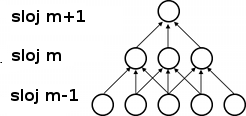
\includegraphics[scale=0.8]{imgs/sparse_1D_nn.png}
\caption{Rijetka povezanost}
\label{fig:sparse-nn}
\end{figure}

Konvolucijski slojevi iskorištavaju lokalnu korelaciju (jedan neuron utječe samo na bliske susjede), što znači da je neuron $m-1$ sloja povezan samo sa prostorno bliskim neuronima $m$-tog sloja. Na slici \ref{fig:sparse-nn} je primjer lokalnog povezivanja širine 3 neurona za jednodimenzijski ulaz.
Neka je $m-1$ sloj ulazni sloj. Tada je vidno polje neurona u sloju m široko 3 s obzirom na ulaz. Neuroni u sloju $m+1$ su isto povezani s 3 neurona iz prošlog sloja, ali ako se gledaju s obzirom na ulazni sloj, onda je njihovo vidno polje široko 5 neurona. Arhitektura mreže tako ograničava takve ''filtere'' na lokalni uzorak (budući da ne reagiraju na druge dijelove ulaza). Slaganje više takvih slojeva omogućava da ''filteri'' polako postaju globalni (odnosno prostiru se preko većeg broja ulaznih piksela). Na primjer, neuron u sloju $m+1$ može predstavljati \engl{encode} nelinearnu značajku duljine 5.

\begin{figure}[htb]
\centering
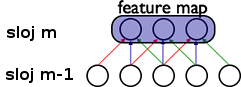
\includegraphics{imgs/conv_1D_nn.png}
\caption{Zajedničke težine}
\label{fig:conv-nn}
\end{figure}

Budući da se govori o primjeni u računalnom vidu, ulazi su uglavnom 2D slike.
Ulaz u konvolucijski sloj ima dimezije $x * y * r$, gdje je $x$ širina slike, $y$ visina slike, a $r$ je broj kanala (konkretno za RGB sliku je $r = 3$). Dimenzionalnost konvolucijskog sloja ne ovisi direktno o ulaznom sloju, već samo o broju kanala i iznosi $d * d * r * k$, gdje je $d$ širina odnosno visina filtera za konvoluciju, $r$ je broj kanala prethodnog sloja, $k$ je broj mapa značajki trenutnog sloja (ekvivalent broju kanala na ulazu). Primjer takvog sloja ima filter dimenzija $7 * 7$ i 20 mapa značajki što daje $7 * 7 * 3 * 20 = 2940$ težina (značajno manje od prije spomenutih 10 milijuna). Naravno, broj mapa značajki se zna penjati i do nekoliko stotina, no broj težina je i u tom slučaju smanjen naspram potpuno povezanog skrivenog sloja.

Gledano s drugog stajališta, neuroni koji čine konvolucijski sloj dijele zajednički vektor težina $\boldsymbol{w}$ i pomak $b$. Time se omogućava da se neka značajka otkrije bez obzira na njezinu lokaciju u ulaznom prostoru. Ova je tehnika vrlo efikasna jer uvelike smanjuje broj parametara sloja, pa time i broj parametara koji se treniraju. I \emph{gradijentni spust} se još uvijek može koristiti za učenje parametara. Slika \ref{fig:conv-nn} prikazuje takav sloj. Težine iste boje su zajedničke neuronima.

U praksi se mapa značajki računa na način da se ulazna slika konvoluira sa linearnim filtrom, doda se pomak $b$ i na dobiveni rezultat primjeni aktivacijska funkcija (aktivacijske funkcije opisane su u poglavlju \ref{chap:aktivacijske_funkcije}).

\begin{equation}
h_{ij}^k = f((\boldsymbol{w}^k * \boldsymbol{x})_{ij} + b_k)
\label{eq:feature_map}
\end{equation}


\subsection{Aktivacijske funkcije}
\label{chap:aktivacijske_funkcije}

Kod logističke funkcije je spomenuto da rezultati množenja ulaza s težinom i zbrajanja s pomakom prolaze još i kroz izlaznu funkciju. Naziv za tu izlaznu funkciju u kontekstu neuronskih mreža je aktivacijska funkcija.
Kod logističke regresije aktivacijska funkcija je logistička sigmoid funkcija (formula \ref{eq:logisticka_funkcija}, slika \ref{fig:logistic_sigmoid}) zbog koje je izlaz logističke regresije probabilistički. Logistička funkcija je nelinearna, monotono rastuća funkcija čiji se izlaz asimptotski približava nekoj konačnoj vrijednosti (na primjer, broju 1) dok ulaz raste prema $\pm \inf$. Zbog tih svojstava MLP (poglavlje \ref{chap:viseslojni_perceptron}) može aproksimirati proizvoljnu nelinearnu funkciju.

\begin{figure}[htb]
\centering
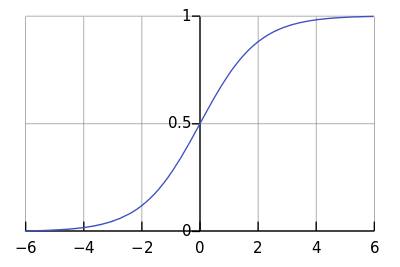
\includegraphics[width=240px]{imgs/logistic_curve.png}
\caption{Logistička sigmoid funkcija}
\label{fig:logistic_sigmoid}
\end{figure}

Osim standardne sigmoid funkcije definirane formulom:
\begin{equation}
f(x) = \frac{1}{1+e^{-x}}
\label{eq:logisticka_funkcija}
\end{equation}
često se koristi i hiperbolna tangent funkcija $f(x) = \tanh(x)$ (slika \ref{fig:tanh_plot}), isto iz porodice logističkih funkcija.

\begin{equation}
f(x) = \tanh(x) = \frac{\sinh(x)}{\cosh(x)} = \frac{e^{x} - e^{-x}}{e^{x} + e^{-x}} = \frac{e^{2x} - 1}{e^{2x} + 1} = \frac{1 - e^{-2x}}{1 + e^{-2x}}
\label{eq:tanh_def}
\end{equation}
Hiperbolna tangent funkcija se više preferira kao aktivacijska funkcija iz istog razloga zbog kojeg se ulazi normaliziraju: pokazalo se (LeCun u radu \cite{lecun-98b}) da mreže brže konvergiraju ako su ima ulazi normalizirani (translatirani tako da im je srednja vrijednost 0 i standardna deviacija 1). Izlazi jednog sloja su ulaz u drugi iz čega slijedi da bi i izlazi trebali biti u prosjeku oko nule, što se postiže $\tanh$ funkcijom, dok su izlazi sigmoid funkcije pozitivni i centrirani oko 0.5 (ili neke druge pozitivne vrijednosti, ovisno o konkretnom obliku funkcije).

\begin{figure}[htb]
\centering
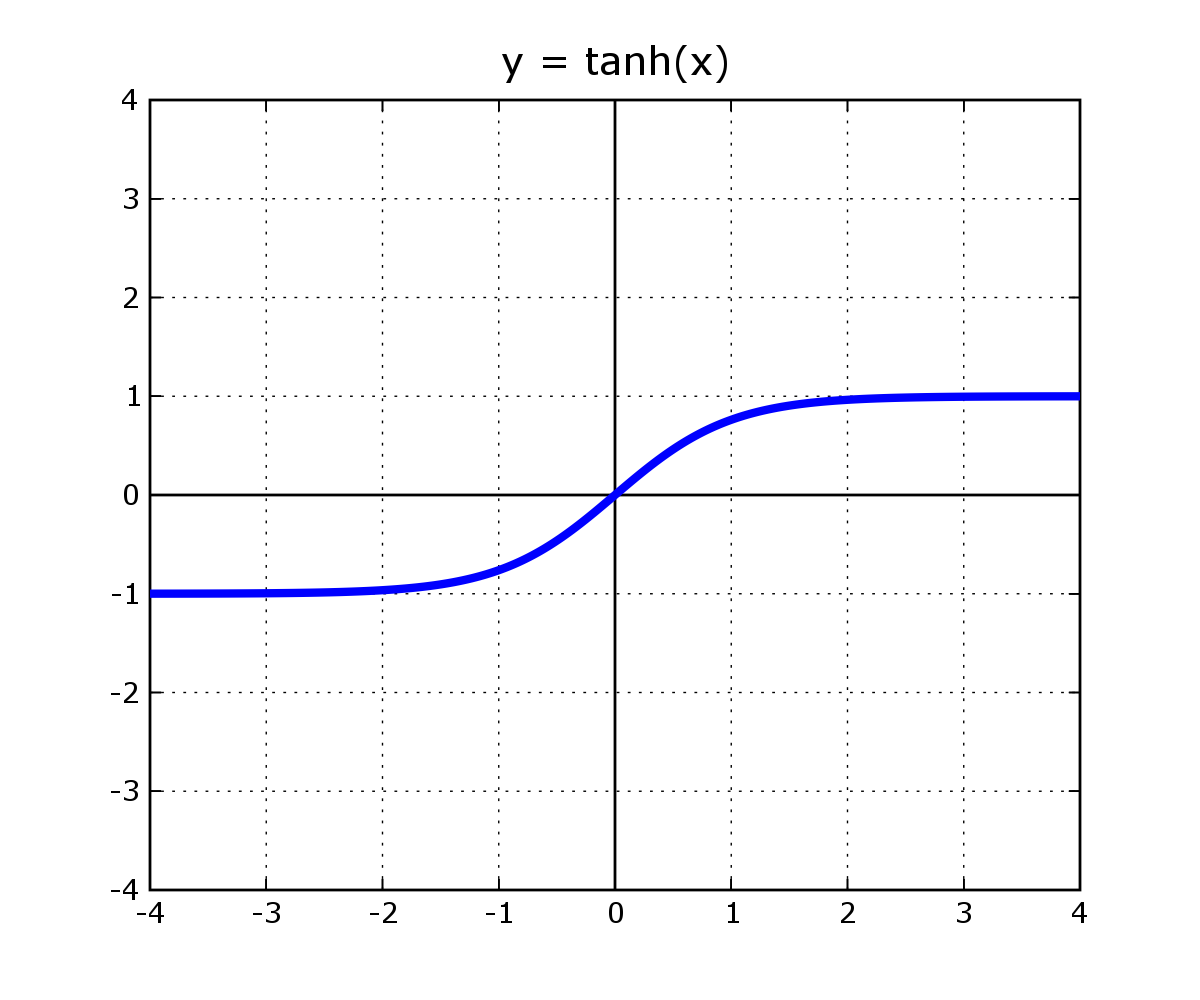
\includegraphics[width=250px]{imgs/tanh_plot.png}
\caption{Hiperbolna tangent funkcija}
\label{fig:tanh_plot}
\end{figure}

Autor u radu \cite{lecun-98b} preporuča korištenje logističke funkcije $f(x) = 1.7159 tanh(\frac{2}{3} x)$. Konstante u navedenoj funkciji su odabrane tako da, ako je ulaz normaliziran, izlazi će isto imati varijancu blizu 1. Konkretni sigmoid ima i sljedeća svojstva: (a) $f(\pm 1) = \pm 1$, (b) druga derivacija ima maksimum u točki $x = 1$.

Logističke funkcije u svojim izrazima često sadrže potencije prirodnog logaritma na neku realnu potenciju $e^{x}, x \in R$, što je računalno prilično zahtjevno. Taj se problem rješava aproksimacijom konkretnog izraza polinomijalnog funkcijom.

% http://web.stanford.edu/~awni/papers/relu_hybrid_icml2013_final.pdf
Drugi je problem nestajući gradijent \engl{vanishing gradient problem}. Nestajući gradijent je pojava koja se događa kada neuroni nekog sloja duboke neuronske mreže imaju gradijente blizu nule jer su izlazi sloja bili blizu zasićenja, odnosno blizu asimptota (koje su često $\pm 1$). Gradijenti blizu nule uzrokuju sporu konvergenciju jer malen iznos gradijenta znači i malu promjenu težina, a pokazalo se i da takve mreže često zaglave u lokalnim minimumima.

\emph{Rectified linear unit} (kraće ReLU) je vrsta aktivacijske funkcije definirana formulom:
\begin{equation}
f(x) = max(0, x) =
    \left\{
        \begin{array}{ll}
            0  & \mbox{ako } x < 0 \\
            x  & \mbox{ako } x \geq 0
        \end{array}
    \right.
\end{equation}
ReLU rješava oba gore navedena problema: brzo se računa, kao i gradijent (koji je 1, ako je $x > 0$ ili 0) i gradijent nikad ne uđe u zasićenje (uvijek je 1 ili 0), neovisno o dubini mreže.

No, ReLU-ovi imaju i potencijalne mane: ako neki neuron nije aktivan, gradijent je 0, što znači da se težine tog neurona više ne mogu pomaknuti gradijentnom optimizacijom. Tome se problemu može doskočiti postavljanjem početnog pomaka \engl{bias} na neku malu pozitivnu vrijednost (na primjer 0.001), čime će na početku svi neuroni biti aktivirani. Gradijentna optimizacija ih tada može pomicati prema ishodištu (praktički isključiti) ili u pozitivnom smjeru. \cite{maas2013rectifier}

Vjerovalo se i da dobri rezultati, koje ReLU aktivacije postižu u dubokim neuronskim mrežama, potiču i od mogućnosti da ReLU aktivacijska funkcija ''isključi'' neuron (ako vrijednost na ulaza u aktivaciju postane < 0). Rad \cite{xu2015empirical} je pokazao da uspjeh ReLU-a ne leži u gašenju nekih neurona (implicitnom uvođenju rijetke povezanosti). U radu je dana usporedba standardne ReLU funkcije, \emph{leaky ReLU} (lReLU) funkcije, \emph{parametric ReLU} (PRelU) funkcije i \emph{randomized ReLU} (RReLU) funkcije. Eksperimenti su pokazali da funkcije bez nagiba sa smjerom 0 (praktički sve osim standardnog ReLU-a), konstantno daju bolje rezultate što znači da teorija o gašenju neurone ne vrijedi, jer takve funkcije nikad potpuno ne gase neurone. Pokazano je i da (na manjem skupu podataka) korištenje determinističkog nagiba, ili učenje nagiba na temelju podatka može uzrokovati prenaučenost, naspram funkcije sa slučajnim odabirom nagiba (nagib iz nekog raspona vrijednosti).

\begin{figure}[htb]
\centering
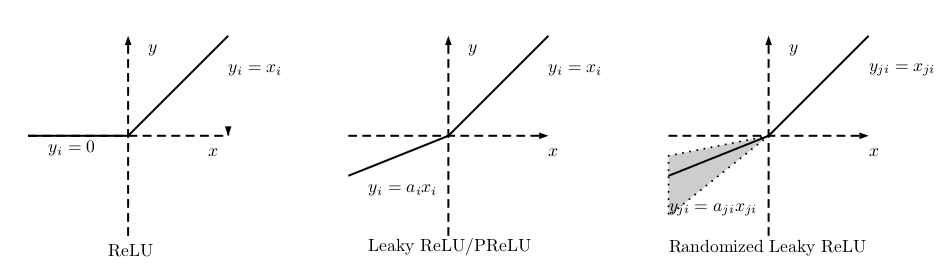
\includegraphics[width=\textwidth]{imgs/relus.png}
\caption{Usporedba ReLU aktivacijskih funkcija}
\label{fig:relu_plot}
\end{figure}

\subsection{Sažimanje}

Sažimanje maksimalnog odziva je vrsta nelinearnog poduzorkovanja gdje se ulazna slika dijeli na više nepreklapajućih pravokutnika i za svaki pravokutnik vrati se najveća vrijednost.

On je važan u računalnom vidu iz dva razloga:
\begin{enumerate}
    \item smanjuje računsku složenost za gornje slojeve
    \item povećava neosjetljivost na translacije u slici
\end{enumerate}

Pojasnimo malo povećanje neosjetljivosti na translacije: recimo da se radi sažimanje maksimuma nad regijom od 2x2 piksela. Neka je gornji lijevi piksel onaj s maksimalnom vrijednošću. Ako se sve na slici pomakne za jedan piksel udesno, piksel s maksimalnom vrijednošću će biti gornji desni. To znači da će u oba slučaja izlaz sloja sažimanja maksimuma biti jednak, tj biti će neosjetljiv na takve translacije.

Uobičajena je praksa da se u gornjim slojevima povećava broj mapa značajki. Time bi računalna složenost previše ekspandirala u višim slojevima. Budući da viši slojevi sadrže informacije visoke razine \engl{high level information}, nije važno da su takve informacije dostupne za svaki piksel, dovoljno je da one pokrivaju veće regije slike. Iz tog razloga se poduzorkovanjem u višim slojevima ne gube važne informacije, a uvelike se smanjuje broj operacija i vrijeme potrebno za računanje mapa značajki.

\subsection{Primjer arhitekture}

LeCun je još 1989. godine u radu \cite{lecun-98b}, za klasifikaciju rukom pisanih brojeva na poštanskim pošiljkama, predstavio konvolucijsku mrežu čija arhitektura je začetak današnjih arhitektura. Takva mreža imala je 3 konvolucijska sloja, bez slojeva sažimanja maksimumom, s potpuno povezanim slojem na kraju. Značajan je i LeCun-ov rad \cite{gradient_document} u kojem se predstavlja arhitektura nazvana LeNet, čije inačice se koriste u mnogim verzijama konvolucijskih mrežama.

\begin{figure}[htb]
\centering
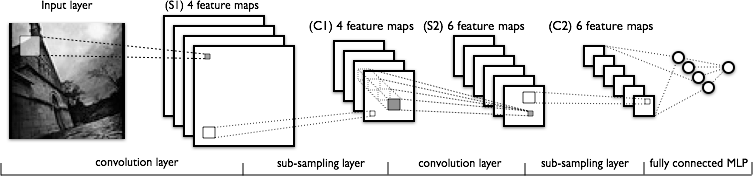
\includegraphics[width=\textwidth]{imgs/mylenet.png}
\caption{LeNet mreža}
\label{fig:lenet5}
\end{figure}
%(slika http://deeplearning.net/tutorial/_images/mylenet.png)

U početnim se slojevima mreže izmjenjuju slojevi sažimanja maksimalnog odziva i mape značajki. Konkretno, prvi sloj se sastoji od 4 mape značajki, zatim slijedi sloj sažimanja maksimuma, pa sloj od 6 mapi značajki i opet sloj sažimanja maksimuma. Zadnji dio takve mreže je višeslojni perceptron na čije su ulaze spojeni izlazi zadnjeg sloja sažimanja maksimuma. Taj se višeslojni perceptron sastoji od 2 sloja. Prvi je skriveni sloj, a iza njega je sloj logističke regresije. Logistička regresija na kraju čini konačnu klasifikaciju. U konkretnom primjeru postoji 10 izlaza, jedan za svaku znamenku.

\chapter{Učenje mreže}

''Učenjem'' modela naziva se postupak pronalaska optimalnih parametara modela. Optimalni parametri su oni koji danim modelom modeliraju skup podataka za učenje, $\mathcal{D}$. No, modeli se često znaju prilagoditi skupu podataka za učenje pa se zapravo relevantni rezultati dobivaju kad se model testira na neviđenim podacima.

Rješenje za optimalne parametre neuronskih mreža nije dostupno u zatvorenoj formi pa se poseže za gradijentnim metodama koje onda kroz iteracije pronalaze optimalne parametre. To znači da nam je potrebna ciljna funkcija, funkcija čiji rezultat nam govori koliko su parametri modela dobri.

Budući da se i semantička segmentacija na neki način može gledati kao klasifikacija, jer se na kraju svaki piksel ili grupa piksela neke slike klasificiraju (za razliku od klasifikacije gdje svaki ulaz ima jednu oznaku, u semantičkoj segmentaciji svaka slika ima skup oznaka koje je potrebno predvidjeti), prvo što pada na pamet je jedan-nula funkcija gubitka. Ako model preslikava ulazni primjer u jedan od razreda iz skupa ${0, ..., L}$, definirajmo takvo preslikvanje funkcijom f $f: R^D \rightarrow {0, ..., L}$, onda se funkcija gubitka može definirati kao:
\begin{equation}
\ell_{0, 1} = \sum_{i = 0}^{\abs{\mathcal{D}}} I_{f(x^{(i)}) \neq y^{(i)}}
\end{equation}
gdje je $\mathcal{D}$ skup podataka, a $I$ indikatorska funkcija definirana kao:
\begin{equation}
I(x) =
    \left\{
	    \begin{array}{ll}
		    1  & \mbox{ako je x istinit} \\
		    0  & \mbox{inače}
	    \end{array}
    \right.
\end{equation}

No, budući da jedan-nula gubitak nije derivabilan pa je nemoguće provoditi metode gradijentnog spusta, on nije praktičan za korištenje. Stoga se uvodi funkcija negativne log izglednosti \engl{negative log likelihood}, spomenuta u poglavlju \ref{chap:logisticka_regresija}.
\begin{equation}
NLL(\theta, \mathcal{D}) = - \sum_{i = 0}^{\abs{\mathcal{D}}} \log P(Y = y^{(i)} | x^{(i)}, \theta)
\end{equation}

\section{Algoritam unazadne propagacije, engl. backpropagation}
Općeniti opis, formula, primjer. Prilagodba za konvolucijski sloj.

\section{Gradijentni spust}
Motivacija, definicija, vrste gradijentnih spusteva.

\subsection{Stohastički gradijentni spust}
Prednosti, nedostaci, razlika

\subsection{RMS prop}
Motivacija, varijante RMS propa, 
prednosti, nedostaci

\subsection{Resilient propagation (RProp)}
Opis, prednosti, nedostatci, varijente (Rprop+, Rprop-)

\section{Regularizacija}
Regularizacija je često korištena tehnika u strojnom učenju, a odnosi se na postupak pružanja dodatnih informacija funkciji gubitka kako bi se rješio problem šuma u ulaznom skupu podataka i problem prenaučenosti. Prenaučenost je pojava tokom učenja modela kad se model prilagodi skupu za učenje u tolikoj mjeri da točnost na skupu za provjeru \engl{validation set} počne padati, iako se točnost na skupu za učenje povećava.

Regularizacijom se sprječava da se model previše prilagodi skupu za učenje tako da pogreška na neviđenim podacima bude manja (skupu za provjeru) iako se pogreška na skupu za učenju još može smanjiti. U idućim poglavljima navedene su najčešće tehnike za regularizaciju modela dubokih neuronskih mreža.

\subsection{$L_1$ i $L_2$ regularizacija}
$L_1$ norma je suma apsolutnih iznosa kartezijevih komponenti vektora. Drugačije gladajući, $L_1$ norma se definira kao suma projekcija vektora na koordinatne osi. Za neki vektor $\boldsymbol{x}$ se $L_1$ norma definira kao:
\begin{equation}
\norm{\boldsymbol{x}}_1 = \sum_{i = 1}^{n} \abs{x_i}
\end{equation}

$L_2$ norma je suma kvadrata komponenti vektora. Za neki vektor $\boldsymbol{x}$ se ona definira:
\begin{equation}
\norm{\boldsymbol{x}}_2 = \sum_{i = 1}^{n} {x_i}^2
\end{equation}

Tokom učenja modela, želimo modelom što bolje modelirati podatke nad kojima učimo, no pravi je cilj da model radi dobro na neviđenim primjerima (primjeri koje nije vidio tokom učenja). Pojasnimo na primjeru logističke regresije što se događa ako učenje predugo traje: budući da funkcija negativne log izglednosti asimptotski teži prema nuli, optimizacija nikada neće završiti, a dogodit će se da neke težine u mreži stalno rastu jer tim rastom uzrokuju polagano padanje negativne izglednosti na skupu za učenje. Jednaka stvar se događa i u neuronskim mrežama, gdje je broj težina još puno veći.

Tom rastu se može doskočiti tako da se norma vektora uključi u funkciju gubitka. Funkcija $R$ označava normu vektora težina mreže. Regularizirana funkcija gubitka je onda:
\begin{equation}
    E(\theta, \mathcal{D}) = NLL(\theta, \mathcal{D}) + \lambda R(\theta) = \\
    = NLL(\theta, \mathcal{D}) + \lambda \norm{\theta}_p^p
\end{equation}
gdje je
\begin{equation}
    \norm{\theta}_p = (\sum_{j = 0}^{\abs{\theta}} \abs{\theta_j}^p)^{\frac{1}{p}}
\end{equation}
$p$ je najčešće 1 ili 2, odnosno koristi se $L_1$ ili $L_2$ norma. $\lambda$ je regularizacijski faktor, jedan od hiperparametara mreže, koji se određuje eksperimentalno.

\subsection{Slučajne transformacije ili Umjetno povećanje skupa za učenje}

Kod modela s velikim brojem parametara, kao što su duboke neuronske mreže, veličina skupa za učenje uvelike utječe na rezultate: što je veći skup za učenje, to su bolji rezultati. No, taj je broj uvijek ograničen. Kod semantičke segmentacije broj podataka je još više ograničen jer je sam postupak označavanja slika semantičkim oznakama dugotrajan pa time i skup.
Zato se provodi postupak umjetnog ''povećanja'' skupa za učenja slučajnim transformacijama.

Kod računalnog vida, koji se većinom bavi slikama, slučajne transformacije su obično:
\begin{itemize}
  \item
  	\textbf{translacije} slike po x ili y osi za neki malen pomak, na primjer 5 \% slike
  \item
    \textbf{rotacije} slike za kut od $\pm 7\deg$
  \item
  	\textbf{skaliranje} (uvećavanje ili smanjivanje) slike za neki faktor koji je obično u raponu od <0.9, 1.1>
  \item
    \textbf{smik} slike za kut od$\pm 5\deg$
\end{itemize}

Slučajne transformacije se koriste tako da se za svaku sliku prvo odabere podskup filtera koji će se koristiti na toj slici, a zatim se slučajno odabiru parametri svakog od odabranih filtera.

Jedan način korištenja je da se pomoću navednih funkcija unaprijed generira povećana verzija skupa podataka, a drugi da se transformacije sprovode ''uživo'', odnosno prije svake epohe treniranja. Tokom provođeja transformacija ''uživo'' mreža se nikad ne trenira s istom slikom dva puta. Svaki put mreža ''vidi'' drugu verziju (transformiranu) iste slike čime se uvelike sprječava pretreniranost i prevelika prilagodba na skup za učenje.

\subsection{Dropout}

Točnost predikcije raznih modela čije treniranje počinje sa slučajno inicijaliziranim parametrima, se povećava ako se koristi prosjek predikcija više istrenranih modela. Takav način korištenja gotovih modela se naziva uprosječivanje modela \engl{model averaging}. No, mane takvog pristupa su (i )što treniranje svake mreže traje dugo i (ii) ne želimo tokom korištenja pokretati više modela za isti primjer jer to opet dugo traje što je pogotovo loše za primjenu u realnom vremenu.

\emph{Dropout} je metoda za učinkovito uprosječivanje modela velikih neuronskih mreža\cite{hinton_dropout}. Uzmimo za primjer jedan skriveni sloj na kojem čemo primjeniti \emph{dropout} metodu. Svaki puta kad mreži na ulaz postavimo jedan primjer iz skupa za učenje, slučajno ''ugasimo'' svaki neuron s vjerojtnošću $p$ (za skrivene slojeve najčešće je $p = 0.5$, odnosno ''ugasimo'' polovicu neurona. ''Gašenjem'' se smatra postavljanje izlaza određenog neurona na 0. To zapravo znači da slučajno odabiremo jednu od $2^H$ arhitektura mreže, gdje je $H$ broj neurona u skrivenom sloju, a sve arhitekture dijele iste težine. Dijeljenje težina između velikog broja arhitektura, odnosno modela, je zapravo jaka regularizacija mreže. Budući da postoji velik broj arhitektura, svaka će pojedina arhitektura vidjeti samo nekolicinu primjera.

Ostaje još za odgovoriti što se događa tokom testiranja modela (ili korištenja). Prva ideja je odabrati nekoliko različitih arhitektura, napraviti njihove predkcije i uprosječiti ih. No, brži način je koristiti sve neurone skrivenog sloja, a njihove izlaze onda pomnožiti s $p$. Može se pokazati da je to jednako računanju geometrijske sredine predikcije svih $2^H$ modela.

Kod mreža s više slojeva, \emph{dropout} kod ulaznih slojeva je manji, koristi se $p = 0.9$ (samo 10\% ulaznih neurona se gasi). Neki autori navode da koriste u svim skrivenim slojevima $p = 0.5$, dok neki postepeno smanjuju $p$ od 0.9 (na ulazu), do 0.5 u zadnjem skrivenom sloju.

Ako se duboka mreža lako prenauči, \emph{dropout} će osjetno smanjiti grešku. No, ako se mreža ne može prenaučiti, onda je potrebno koristiti mrežu s više parametara (širu ili dublju).
% Hinton: nips2012_hinton_networks_01.pdf

\section{Stopa učenja}
Kako utječe na učenje, kad mijenjati, kako.

\section{Uvjeti zaustavljanja}
Načini određivanja trenutka zaustavljanja

\chapter{Semantička segmentacija}
Definicija semantičke segmentacije

\section{Opis}
primeri, slike

\section{Primjene}
Motivacija?

\section{Testni skupovi}
Skupovi podataka korišteni u evaluaciji.

\subsection{Stanford Background Dataset}
Vrste oznaka, veličine slika, zastupljenost oznaka - histogram

\subsection{SIFT Flow}
Vrste oznaka, veličine slika, zastupljenost oznaka - histogram
Standardni dataset, popis rezultata

\chapter{Rezultati}
TODO

\section{Mjere}
Pixel accuracy, mean class accuracy, IOU (intersection over union).

\chapter{Zaključak}
Zaključak.

\bibliography{literatura}
\bibliographystyle{fer}

\begin{sazetak}
Sažetak na hrvatskom jeziku.

\kljucnerijeci{računalni vid, neuronske mreže, konvolucijske mreže, duboko učenje, semantička segmentacija}
\end{sazetak}

% TODO: Navedite naslov na engleskom jeziku.
\engtitle{Semantic segmentation of outdoor scenes using deep neural networks}
\begin{abstract}
Abstract.

\keywords{computer vision, neural networks, convolutional networks, deep learning, semantic segmentation}
\end{abstract}

\end{document}